%%%%%%%%%%%%%%%%%%%%%%%%%%%%%%%%%%%%%%%%%%%%%%%%%%%%%%%%%%%%%%%%%%%%%%%%%%%%%%%%
%
% LICENZA
%
% Quest'opera è stata rilasciata sotto la licenza
% Creative Commons Attribution-NonCommercial-ShareAlike 2.5 Italy.
% Per leggere una copia della licenza visita il sito web
% http://creativecommons.org/licenses/by-nc-sa/2.5/it/
% o spedisci una lettera a Creative Commons, 171 Second Street, Suite 300, San
% Francisco, California, 94105, USA.
%
% This work is licensed under the Creative Commons
% Attribution-NonCommercial-ShareAlike 3.0 Unported License. To view a copy of
% this license, visit http://creativecommons.org/licenses/by-nc-sa/3.0/ or send
% a letter to Creative Commons, 171 Second Street, Suite 300, San Francisco,
% California, 94105, USA.
%
% For info send a mail to pietro.giuffri@gmail.com
%
%%%%%%%%%%%%%%%%%%%%%%%%%%%%%%%%%%%%%%%%%%%%%%%%%%%%%%%%%%%%%%%%%%%%%%%%%%%%%%%%

\documentclass[a4paper,12pt,oneside]{article}
\usepackage[T1]{fontenc}
\usepackage[utf8]{inputenc}
\usepackage[italian]{babel}

\usepackage[font=small,format=hang]{caption}
\usepackage{graphicx}

\usepackage{listings}
\usepackage{fourier}

\usepackage[bookmarksnumbered,colorlinks]{hyperref}
\usepackage{breakurl}
\usepackage{guit}

\lstset{basicstyle=\small\ttfamily,
  keywordstyle=\color{blue},
  commentstyle=\color{red},
  stringstyle=\color{green},
  frame=lines,
  breaklines = true, % per mandare a capo le righe troppo lunghe
  breakautoindent = true, % indenta le righe spezzate
  breakindent = 30pt, % indenta le righe di 30pt
  language=bash,
  showspaces=false,
  showstringspaces=false,
  showtabs=false,
  emph={touch,mkdir,echo,rm},
  emphstyle=\color{blue}
}

\begin{document}
\title{git4\LaTeX \\
  Una guida introduttiva a Git per progetti \LaTeX}
\author{Pietro Giuffrida}
\maketitle
\clearpage
\tableofcontents
\clearpage
\section{Scopo della guida}
Git è un \emph{revision control system} (o \emph{version control system}, spesso
abbreviato in VCS), vale a dire un programma che permette di tener traccia di
tutte le modifiche e le evoluzione effettuate nel corso della stesura di un
codice o di un qualsiasi progetto su supporto digitale. Git è rilasciato sotto
licenza GPL, ed è disponibile, oltre che nei repository delle varie distribuzioni
GNU-Linux, all'indirizzo \url{http://git-scm.com/}.

\LaTeX{} è un programma di composizione tipografica di alta qualità. \LaTeX{} è
software libero. Generalmente fa parte dei programmi fondamentali preinstallati in
ogni distribuzione GNU-Linux, ed è comunque disponibile a partire dall'indirizzo
\url{http://www.latex-project.org/} per i principali sistemi operativi.

In questo documento desidero mostrare come utilizzare Git per tener traccia
delle modifiche rilevanti e delle versioni elaborate nel corso dell'elaborazione
di un documento scritto con \LaTeX. Tramite Git è infatti possibile mantenere un
backup incrementale del proprio codice sorgente, sia in locale che in remoto,
senza incorrere in un eccessivo dispendio di energie e senza deconcentrarsi
eccessivamente dalla stesure del proprio testo. I passaggi descritti
relativamente all'uso di Git dovrebbero essere validi in linea di principio per
l'elaborazione di qualsiasi documento (foto, file \lstinline|.doc|, \lstinline|.xls|
e quant'altro), ma Git dà il meglio di sé con i file di testo puro, poiché permette
di vedere tutte le modifiche apportate al file di volta in volta. Proprio per questo
l'uso principale di Git, e dei VCS in generale, è quello di controllare lo sviluppo
dei software.\footnote{Git, infatti, è stato creato da Linus Torvalds, inventore
  del kernel Linux, perché aveva bisogno di un buon VCS per gestire lo sviluppo
  di Linux.} Anche il codice dei documenti \LaTeX{} si scrive su file di testo
puro e quindi Git è particolarmente adatto a essere utilizzato in accoppiata con
\LaTeX. Questa guida è proprio strutturata in modo specifico per illustrare la
loro interazione, almeno a livello base.

Solo i primi due paragrafo sono indispensabili. In essi vengono tratte le basi
del funzionamento di Git e  mostrati i passaggi fondamentali per la creazione di
un repository locale del proprio progetto, per il salvataggio progressivo delle
versioni, e quindi per svolgere eventuali operazioni di ripristino.

I paragrafi successivi sono invece dedicate alla creazione e alla
sincronizzazione di un repository remoto (che si tratti di un servizio on-line
o semplicemente di una memoria esterna), e a uno script bash che permette di
eseguire dei commit automatici a ogni salvataggio dei file.

La guida non si prefigge alcun compito specifico per quanto riguarda \LaTeX, a
proposito del quale esistono numerose guide.\footnote{Si veda a questo proposito,
  oltre alla documentazione reperibile sul proprio computer mediante il comando
  \lstinline|texdoc nomepacchetto|, la documentazione in italiano reperibile a
  partire dal sito del \guit\ (\url{http://www.guit.sssup.it}), oltre all'ottima guida
  di L. Pantieri disponibile sul sito
  \url{http://www.lorenzopantieri.net/LaTeX.html}.}

La guida non contempla l'uso di alcuna interfaccia grafica (GUI). Tutti i
comandi e i passaggi illustrati sono eseguiti tramite una shell Unix. Spesso
indicheremo i comandi da eseguire nel seguente modo:
\begin{lstlisting}
~/progetto$ git log -4 -p -- main.tex
\end{lstlisting}
Il carattere \lstinline|$| rappresenta il \emph{prompt} del terminale, cioè
l'invito a inserire un nuovo comando. Ciò che si trova alla sinistra del
\emph{prompt} è il percorso della cartella in cui il comando viene eseguito. In
genere questo percorso è puramente esemplificativo e può essere ignorato. Tutto
ciò che si trova alla destra del \emph{prompt} è il comando vero e proprio che
dovrà essere eseguito dall'utente. Dunque, nell'esempio precedente il comando va
eseguito copiando, o riscrivendo, in un terminale
\lstinline|git log -4 -p -- main.tex| e premendo il tasto Invio. Fra parentesi
ad angolo \lstinline|<...>| sono riportate le parti di un comando che non devono
essere ricopiate così come sono ma andranno sostituite dall'utente, come
spiegato nella guida di volta in volta.

Non ho esperienza né di Git né di \LaTeX{} su sistemi operativi non
Unix-like. Un minimo di compatibilità con altri sistemi è garantita dal fatto
che i comandi tipici della shell Unix sono evidenziati e commentati, in modo
che l'utente di altri sistemi operativi o abituato all'uso di GUI possa
sostituirli svolgendo altrimenti le medesime attività. I comandi di Git
dovrebbero invece restare i medesimi in ogni sistema operativo, per quanto anche
in questo caso le medesime attività possano essere svolte mediante GUI. Nel
paragrafo~\ref{sec:gitwin} è spiegato come installare una versione di Git sui
sistemi operativi Windows.

Non sono un esperto di informatica, ma trovo bello far le cose, per quanto
possibile, con le mie mani, sapere cosa fa la macchina e avere l'illusione che
nel rapporto quasi-simbiotico con il computer sia io a decidere.

Dato il carattere ludico della presente guida, scelgo come licenza la Creative
Commons Attribution-NonCommercial-ShareAlike 2.5 Italy. Gli unici vincoli sono
quindi quelli di riconoscere la paternità dell'opera
originale, di non lucrare sulla sua distribuzione, e di distribuire l'opera e
i suoi eventuali derivati con la medesima licenza.\footnote{
  Quest'opera è stata rilasciata sotto la licenza
  Creative Commons Attribution-NonCommercial-ShareAlike 2.5 Italy.
  Per leggere una copia della licenza visita il sito web
  \url{http://creativecommons.org/licenses/by-nc-sa/2.5/it/}
  o spedisci una lettera a Creative Commons, 171 Second Street, Suite 300, San
  Francisco, California, 94105, USA.}

Per maggiori informazioni sui vari comandi Git illustrati, loro opzioni e
argomenti è possibile consultare la documentazione presene sul proprio computer
eseguendo il comando \lstinline|man git-<comando>| e sostituendo a
\lstinline|<comando>| il comando Git che si vuole approfondire. Così, per
saperne di più su \lstinline|git commit| si dovrà eseguire
\lstinline|man git-commit|.

\section{Introduzione a Git}
\label{sec:introduzione-git}

Git permette di tenere traccia delle modifiche apportate a un progetto registrando
una copia dei file del progetto in un database. Sostanzialmente Git scatta una
foto dei file presenti nella cartella nel momento in cui si effettua il
\emph{commit}.

Per controllare continuamente l'integrità dei dati Git utilizza un sistema, detto
\emph{checksum}, che associa a ogni stato di un progetto una sequenza di bit che
la identifica. Nella fattispecie Git utilizza l'algoritmo SHA-1 che restituisce
una stringa esadecimale (detta \emph{hash}) composta da $40$ caratteri
alfanumerici (numeri da \lstinline|0| a \lstinline|9| e lettere da \lstinline|a|
a \lstinline|f|) che può apparire così:
\begin{lstlisting}
43c5858e91a7090b834dd9f09ddfae1061901ee4
\end{lstlisting}
In questo modo è impossibile modificare un file del progetto senza che Git se
ne renda conto. Per fare riferimento a una particolare versione del progetto
si indica il corrispondente \emph{hash} o, a volte, solo i primi $7$ caratteri.

\begin{figure}
  \centering
  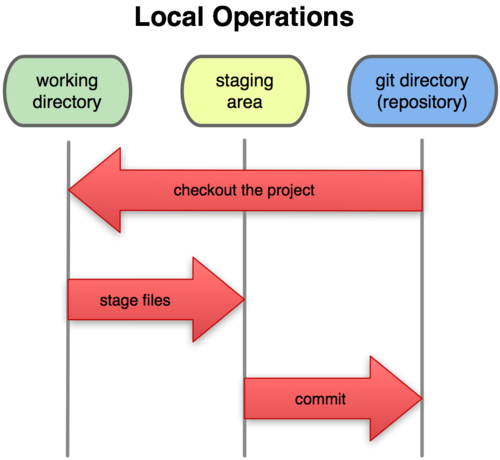
\includegraphics{18333fig0106-tn}
  \caption{Working directory, staging area e git directory. Immagine presa da:
    \url{http://progit.org/book/ch1-3.html}.}
\end{figure}
Prima di iniziare a metterci al lavoro c'è un'ultima cosa da sapere su Git. I
file possono trovarsi in tre stati chiamati, in inglese, \emph{committed},
\emph{modified} e \emph{staged}. \emph{Commited} significa che il file è stato
salvato nel proprio database locale; \emph{modified} indica che il file è stato
modificato ma non ancora salvato nel database con un \emph{commit};
\emph{staged} significa che il file è stato modificato e la sua versione attuale
verrà salvata nel database con il \emph{commit} successivo, cioè è preparato per
essere aggiunto nella nuova revisione. Un progetto Git può quindi essere
suddiviso in tre sezioni principali: la \emph{git directory}, la
\emph{working directory} e la \emph{staging area}. La prima è dove Git conserva
i metadati e gli oggetti del database del proprio progetto. La
\emph{working directory} è, come dice il nome stesso, la ``cartella di lavoro'',
ossia una copia di una versione del progetto a nostra disposizione per l'uso e
la modifica dei file. L'ultima sezione, la \emph{staging area}, è un semplice
file, generalmente contenuto nella cartella Git, che conserva le informazioni su
ciò che dovrà entrare nel \emph{commit} successivo.

Con Git si lavora più o meno così:
\label{list:lavoro-git}
\begin{enumerate}
\item si modifica uno o più file presenti nella \emph{working directory};
\item si aggiunge un suo \emph{snapshot}, cioè una loro copia, nella
  \emph{staging area};
\item si esegue un \emph{commit}, cioè l'operazione con la quale i file vengono
  copiati così come sono presenti alla \emph{staging area} all'interno della Git
  \emph{directory} in maniera definitiva. Al \emph{commit} viene associato
  l'\emph{hash} che identifica univocamente la versione del progetto così
  salvata.
\end{enumerate}
Se una particolare versione di un file si trova nella cartella git è considerato
\emph{committed}. Se è stato modificato e aggiunto alla \emph{staging area} esso
è detto \emph{staged}. Se è stato modificato da quando è stata aperta la cartella
di lavoro ma non ancora aggiunto alla \emph{staging area} allora il file è detto
\emph{modified}.\footnote{Questo paragrafo è stato tradotto in parte da
  \url{http://progit.org/book/ch1-3.html}.}

\section{Un semplice progetto \LaTeX}
Vogliamo sviluppare un documento con \LaTeX, utilizzando Git come VCS.
Git non funziona in modo particolarmente esotico. Si tratta semplicemente di
creare una directory, di posizionare in essa i nostri file \lstinline|.tex| e di
dire a Git di considerare tale directory come un repository.
\subsection{Creazione e inizializzazione del repository}
\begin{lstlisting}
~$ mkdir progetto
~$ cd progetto
~/progetto$ touch np_main.tex
~/progetto$ git init
~/progetto$ git add .
~/progetto$ git commit -am "Inizializzazione del nuovo progetto"
\end{lstlisting}
Vediamo con calma i singoli passaggi. I primi tre comandi servono
rispettivamente per creare la directory (\lstinline|mkdir <nome_directory>|),
per spostarsi al suo interno (\lstinline|cd <nome_directory>|) e per creare
un file vuoto chiamato \lstinline|np_main.tex| (\lstinline|touch <nome_file>|).

I passaggi successivi, eseguiti sempre dati dall'interno della directory, sono
quelli specifici di Git:
\begin{itemize}
\item con \lstinline|git init| creiamo una cartella nascosta chiamata
  \lstinline|.git/| che contiene il nostro repository Git. Questo comando va
  dato solo al momento della creazione di un nuovo \emph{repository} e poi non
  sarà più necessario riutilizzarlo;
\item \lstinline|git add .| aggiunge l'argomento (in questo caso
  `\lstinline|.|', che è un'abbreviazione del percorso della cartella in cui
  siamo posizionati) alla \emph{staging area} del \emph{repository} appena
  creato;
\item con col comando \lstinline|commit -am "nota di versione"| effettuiamo il
  commit che, come detto, salva una copia dei file contenuti nella \emph{staging
    area} all'interno del database. Nel registro delle operazioni effettuate a
  questa operazione risulterà associato il messaggio \lstinline|"nota di versione"|.
\end{itemize}

Così facendo saremo già pronti a lavorare con il nostro editor di fiducia sul
file \lstinline|.tex| appena creato.

Per continuare il lavoro sul nostro documento e registrare i suoi cambiamenti
dobbiamo eseguire le seguenti operazioni (il seguente elenco puntato deve essere
confrontato con quello presente nel paragrafo~\ref{sec:introduzione-git} a
pagina~\pageref{list:lavoro-git}):
\begin{enumerate}
\item si modificano i file del codice sorgente presenti nella con il nostro
  editor di testo di fiducia, oppure se ne aggiungono di nuovi (per esempio
  possono essere aggiunte nuove figure);
\item si aggiungono i file che vogliamo registrare nel successivo \emph{commit}
  alla \emph{staging area} con il comando \lstinline|git add <file>|, dove al
  posto di \lstinline|<file>| va sostituito l'elenco, separato da uno spazio,
  dei file di interesse. Per maggiori informazioni sull'aggiunta di file a un
  progetto Git vedi il paragrafo~\ref{sec:aggiungere-rimuovere-file};
\item si effettua un \emph{commit} con il comando \lstinline|git commit|. A
  questo punto si aprirà l'editor di testo predefinito di Git per l'inserimento
  del messaggio del \emph{commit}. Vedi il
  paragrafo~\ref{sec:configurazioni-basilari} per sapere come configurare
  l'editor predefinito di Git e il paragrafo~\ref{sec:messaggi-commit} per
  maggiori informazioni sui messaggi dei \emph{commit}.
\end{enumerate}
I punti 2 e 3 possono essere eseguiti insieme se si vogliono aggiungere alla
\emph{staging area} tutti i file che risultano \emph{modified} nella
\emph{working directory} utilizzando il comando \lstinline|git commit -a|.

Prima di eseguire un \emph{commit} si possono modificare più file, se ne possono
aggiungere di nuovi o se ne possono cancellare altri. Nel \emph{commit} verranno
memorizzati tutti i cambiamenti presenti nella \emph{staging area} e solamente
quelli, cioè non verranno considerati i file modificati ma non preparati per la
nuova revisione.

\subsubsection{Messaggi dei \emph{commit}}
\label{sec:messaggi-commit}

In Git, a differenza di altri software VCS, è necessario specificare un
messaggio di \emph{commit} non vuoto. Se quando registriamo un nuovo
\emph{commit} con il comando \lstinline|git commit| non specifichiamo un
messaggio con l'opzione \lstinline|-m| si aprirà l'editor di testo associato di
default a Git in cui potremo scrivere il messaggio del \emph{commit}. Se si
utilizza un editor di testo per scrivere il messaggio di un \emph{commit} è
possibile inserire messaggi estesi su più righe. Generalmente si utilizza la
seguente convenzione:
\begin{itemize}
\item nella prima riga del messaggio, che non deve superare i 72 caratteri, si
  inserisce una breve e riassuntiva descrizione del \emph{commit} che si sta
  registrando. Il testo del messaggio in questo primo rigo può non essere
  correttamente formattato, per esempio può essere assente la punteggiatura o un
  corretto utilizzo dei caratteri maiuscoli;
\item si lascia la seconda riga vuota e a partire dalla terza si scrive un
  paragrafo contenente una descrizione più dettagliata delle modifiche
  apportate. Il testo di questo paragrafo deve utilizzare la punteggiatura
  opportuna e i caratteri maiuscoli dove necessario. Anche le righe di questo
  paragrafo non dovrebbero superare i 72 caratteri;
\item si possono inserire altri paragrafi per descrivere ulteriormente le
  modifiche lasciando una riga vuota fra un paragrafo e il successivo e seguendo
  le convenzioni illustrate nel punto precedente.
\end{itemize}

Nei messaggi il carattere \lstinline|#| viene interpretato come carattere di
commento e ha lo stesso utilizzo del carattere \lstinline|%| in \LaTeX, cioè
tutto ciò che in una riga si trova alla destra del carattere \lstinline|#| verrà
ignorato. Si noti che all'apertura dell'editor di testo per la modifica del
messaggio sono presenti, alla fine del file, delle righe di commento contenenti
delle informazioni relative al \emph{commit} che si sta registrando. Queste
righe possono essere ignorate.

\subsection{Aggiungere e rimuovere file del progetto}
\label{sec:aggiungere-rimuovere-file}

Per controllare lo stato di un \emph{repository} Git esiste il comando
\lstinline|git status|. Questo comando ci permette di monitorare costantemente
la situazione di tutti i file e fornisce spesso dei suggerimenti utili (in
lingua inglese) sulle operazioni che possono essere eseguite sui file. Se dopo
aver effettuato un \emph{commit} si sono modificati dei file, l'output di questo
comando sarà qualcosa di simile a ciò che segue
\begin{lstlisting}
# On branch master
# Changes not staged for commit:
#   (use "git add <file>..." to update what will be committed)
#   (use "git checkout -- <file>..." to discard changes in working directory)
#
#	modified:   TODO
#	modified:   git4latex.tex
#
no changes added to commit (use "git add" and/or "git commit -a")
\end{lstlisting}
In questo esempio nella \emph{working directory} sono presenti due file, tutti e
due \emph{modified} ma non \emph{staged}, come ben spiegato da Git. Nell'ultima
riga dell'output Git ci suggerisce anche come aggiungere i file alla
\emph{staging area}, cioè usando i già visti \lstinline|git add <file>| oppure
\lstinline|git commit -a|. Se aggiungiamo il file \lstinline|git4latex.tex| alla
\emph{staging area} l'output di \lstinline|git status| diventerà
\begin{lstlisting}
$ git add git4latex.tex
$ git status
# On branch master
# Changes to be committed:
#   (use "git reset HEAD <file>..." to unstage)
#
#	modified:   git4latex.tex
#
# Changes not staged for commit:
#   (use "git add <file>..." to update what will be committed)
#   (use "git checkout -- <file>..." to discard changes in working directory)
#
#	modified:   TODO
#
\end{lstlisting}
Adesso \lstinline|git4latex.tex| compare nell'elenco dei file che faranno parte
del prossimo \emph{commit}. Ci viene anche suggerito come rimuovere un file
dalla \emph{staging area}, usando \lstinline|git reset HEAD <file>|, ma
riprenderemo questo discorso nel
paragrafo~\ref{sec:annullare-modifiche-non-salvate}. Non è necessario che tutti
i file siano spostati nella \emph{staging area} prima di effettuare un nuovo
\emph{commit}, possiamo spostare solo quelli che vogliamo registrare nella
revisione successiva.

Se dopo aver spostato un file nella \emph{staging area} lo modifichiamo
nuovamente, questo apparirà sia nell'elenco dei file che faranno parte del nuovo
\emph{commit} sia in quello dei file \emph{modified} ma non \emph{staged}
\begin{lstlisting}
# On branch master
# Changes to be committed:
#   (use "git reset HEAD <file>..." to unstage)
#
#	modified:   git4latex.tex
#
# Changes not staged for commit:
#   (use "git add <file>..." to update what will be committed)
#   (use "git checkout -- <file>..." to discard changes in working directory)
#
#	modified:   TODO
#	modified:   git4latex.tex
#
\end{lstlisting}
Succede questo perché Git non ricorda semplicemente l'elenco dei file che sono
pronti per entrare nella nuova revisione, ma memorizza nella \emph{staging area}
una copia del file così com'era al momento dell'esecuzione del comando
\lstinline|git add <file>|. Prima di effettuare il \emph{commit} quindi è bene
controllare che il file sia solo fra quelli \emph{to be committed} e non anche
fra i file \emph{not staged for commit}, per evitare di inserire nel
\emph{commit} un file alla versione sbagliata. Un metodo semplice per rimediare
a questo pericolo è quello di usare \lstinline|git commit -a|, ma questo è
possibile solo se si vogliono aggiungere al \emph{commit} tutti i file che
risultano \emph{modified}.

Il comando \lstinline|git add| permette di aggiungere al \emph{repository}
qualsiasi file presente nella \emph{working directory}, anche quelli non ancora
conosciuti da Git.\footnote{In effetti subito dopo aver creato il
  \emph{repository} con \lstinline|git init|, Git non conosceva nessun file, noi
  glieli abbiamo presentati con \lstinline|git add <file>|.} Per esempio, se
abbiamo creato un file per la bibliografia, chiamato
\lstinline|bibliografia.bib|, del nostro documento la situazione sarà la
seguente
\begin{lstlisting}
$ git status
# On branch master
# Untracked files:
#   (use "git add <file>..." to include in what will be committed)
#
#	bibliografia.bib
nothing added to commit but untracked files present (use "git add" to track)
\end{lstlisting}
I file \emph{untracked} sono quelli non ancora seguiti da Git poiché non ancora
conosciuti. Come avrete probabilmente già capito, e come suggerito anche
dall'output del comando, per rendere noto a Git il file dovremo usare
\lstinline|git add bibliografia.bib|. Se avessimo provato a effettuare
direttamente un \emph{commit} con \lstinline|git commit -a| avremmo ottenuto la
seguente risposta
\begin{lstlisting}
$ git commit -am "aggiungo bibliografia"
# On branch master
# Untracked files:
#   (use "git add <file>..." to include in what will be committed)
#
#       bibliografia.bib
nothing added to commit but untracked files present (use "git add" to track)
\end{lstlisting}
Git si sarebbe accorto della presenza del nuovo file, ma non lo avrebbe aggiunto
automaticamente al progetto. D'altra parte, se avesse rilevato delle modifiche
ai file precedentemente aggiunti al progetto, non si sarebbe nemmeno curato di
comunicarci che il nuovo file non è ancora stato aggiunto al progetto. Si
sarebbe infatti limitato a salvare le modifiche ai file che gli abbiamo
precedentemente detto di gestire. Solo con il comando \lstinline|git status|
possiamo controllare con certezza lo stato di tutti i file del
\emph{repository}.

Oltre ad aggiungere file a un \emph{repository} è possibile, naturalmente, anche
rimuoverli. La sintassi è la seguente:
\lstinline[emph={}]|git rm <file>|, in cui a \lstinline|<file>| va
sostituito, come al solito, l'elenco dei file che si vogliono cancellare. Questo
comando elimina il file dalla \emph{working directory} e aggiunge la
cancellazione del file alla \emph{staging area}, ma non crea un nuovo
\emph{commit} che dovrà quindi essere eseguito esplicitamente, senza però aver
bisogno di fare altro. Poiché la cancellazione è memorizzata nella
\emph{staging area}, per rimuovere l'eliminazione accidentale di un file, prima
di effettuare un \emph{commit}, eseguita con
\lstinline[emph={}]|git rm <file>|, possiamo usare
\lstinline|git reset HEAD <file>|. Adesso la modifica è presente solo nella
\emph{working directory} (cioè il file è assente dalla cartella di lavoro), per
ripristinarlo useremo \lstinline|git checkout -- <file>|. Non c'è bisogno di
ricordare a memoria tutte le operazioni per il ripristino del
file,\footnote{Queste operazioni dovrebbero   risultare più chiare dopo avere
  letto il paragrafo~\ref{sec:annullare-modifiche-non-salvate}.} queste infatti
sono suggerite dall'output di \lstinline|git status|.
\begin{lstlisting}
$ git rm bibliografia.bib
rm 'bibliografia.bib'
$ git status
# On branch master
# Changes to be committed:
#   (use "git reset HEAD <file>..." to unstage)
#
#	deleted:    bibliografia.bib
#
$ git reset HEAD bibliografia.bib
Unstaged changes after reset:
M	bibliografia.bib
$ git status
# On branch master
# Changes not staged for commit:
#   (use "git add/rm <file>..." to update what will be committed)
#   (use "git checkout -- <file>..." to discard changes in working directory)
#
#	deleted:    bibliografia.bib
#
no changes added to commit (use "git add" and/or "git commit -a")
$ git checkout -- bibliografia.bib
$ git status
# On branch master
nothing to commit (working directory clean)
\end{lstlisting}

\subsubsection{Ignorare file del progetto: \lstinline|.gitignore|}
\label{sec:ignorare-file}
% TODO: rivedere questa sezione

Come ormai sappiamo bene, per aggiungere dei file alla \emph{staging area}
dobbiamo usare il comando \lstinline|git add <file>|, in cui a
\lstinline|<file>| andrà sostituito l'elenco dei file, separati da uno spazio,
che si vogliono includere nel \emph{commit} successivo. Si può scegliere di
procedere in due modi: aggiungere indiscriminatamente tutti i file della
cartella corrente al progetto che stiamo sviluppando; oppure aggiungere un
singolo file. Nel primo caso dovremmo ripetere il comando già usato in fase di
inizializzazione:
\begin{lstlisting}
$ git add .
\end{lstlisting}
Nel secondo caso aggiungiamo un singolo file:
\begin{lstlisting}
$ git add np_secondary.tex
\end{lstlisting}
Per quanto possa sembrare eccessivo, io preferisco usare il secondo comando. Mi
accade con estrema frequenza di dover aggiungere dei file a un progetto, e
spesso sono fin troppo distratto da quel che sto scrivendo per occuparmi di quel
Git si aspetta da me l'aggiunta indiscriminata di ogni file nella directory al
repository presenta però delle controindicazioni. La più ovvia per chi lavora
con \LaTeX{} è la seguente: nel corso dell'elaborazione di un testo
inevitabilmente si procederà alla generazione del documento in pdf a partire dai
sorgenti; \LaTeX{} provvederà quindi alla generazioni di una serie di file
ausiliari (\lstinline|.toc|, \lstinline|.out|, \dots), nonché di un pdf più o
meno inutile. Se eseguissimo il comando \lstinline|git add .| subito dopo una
compilazione, evidentemente Git aggiungerebbe alla \emph{staging area} anche i
vari file di lavoro, dal pdf, ai file di log. Per ovviare a questo
inconveniente, e continuare pigramente a eseguire \lstinline|git add .|, è utile
creare nella nostra directory di un file denominato \lstinline|.gitignore|.
\begin{lstlisting}
$ echo "*.log" >> .gitignore
$ echo "*.pdf" >> .gitignore
$ echo "*.blg" >> .gitignore
$ echo "*.bbl" >> .gitignore
$ echo "*.aux" >> .gitignore
$ echo "*-blx.bib" >> .gitignore
$ echo "*.out" >> .gitignore
$ echo "*~" >> .gitignore
$ git add .gitignore
$ git commit -am "Aggiunto il file .gitignore"
\end{lstlisting}

Mediante questo file, istruiamo Git a proposito di tutti i file che non fanno
effettivamente parte del progetto, pur essendo presenti nella cartella.  Da
questo momento in poi Git si limiterà a ignorarli, il che ci permette di
eseguire prudenzialmente il comando \lstinline|git add .| prima di ogni
\emph{commit}. Generalmente Git è usato per gestire solo il codice sorgente di
un progetto, sia esso un programma o un documento \LaTeX, quindi è buona norma
aggiungere all'elenco dei file ignorati tutti quei file, ausiliari o di output,
che vengono generati nella fase di compilazione, del programma o documento, ma
che non fanno parte del codice sorgente propriamente detto. Nel caso di un
documento \LaTeX{} saranno i file con estensione, per esempio, \lstinline|.log|,
\lstinline|.aux|, \lstinline|.toc| (per i file ausiliari temporanei) e
\lstinline|.pdf| (per il file di output).

\subsection{Consultare la cronologia}
\label{sec:consultare-cronologia}

In Git è possibile, naturalmente, consultare la cronologia dei \emph{commit}
registrati nel \emph{repository} in uso. Il comando da usare è
\lstinline|git log|. L'output di questo comando, senza ulteriori opzioni, sarà
qualcosa di questo tipo
\begin{lstlisting}
commit 9e1691276ba70443c56c214a52088814a5f25ec5
Author: Pietro Giuffrida <pietro.giuffri@gmail.com>
Date:   Sat Oct 2 19:32:12 2010 +0200

    un po' di pulizia

commit 86ee0a0525dd759bb49308b58cf3e761471a04cd
Author: Pietro Giuffrida <pietro.giuffri@gmail.com>
Date:   Sat Oct 2 19:31:24 2010 +0200

    prime due sezioni

commit 43c5858e91a7090b834dd9f09ddfae1061901ee4
Author: Pietro Giuffrida <pietro.giuffri@gmail.com>
Date:   Sat Oct 2 18:53:30 2010 +0200

    Ho solo iniziato a lavorare
\end{lstlisting}
È possibile muoversi nella cronologia con i tasti freccia. Nella prima riga di
ogni revisione (che inizia con \lstinline|commit|) è riportato l'\emph{hash}
esteso corrispondente, nella seconda l'autore (\lstinline|Author|) del
\emph{commit}, quindi la data di salvataggio (\lstinline|Date|) e il messaggio
descrittivo.

È possibile mostrare solo l'elenco degli ultimi \lstinline|n| \emph{commit}
aggiungendo l'opzione \lstinline|-n|. Dunque per mostrare solo l'ultimo
\emph{commit} possiamo usare il comando \lstinline|git commit -1|. Si può
consultare la cronologia relativa a uno o più specifici file e non all'intero
\emph{repository} passando come argomento del comando l'elenco dei file di
interesse, separati da uno spazio: \lstinline|git log -- <file>|. Se si vuole
visualizzare solo l'elenco degli ultimi \lstinline|n| \emph{commit} relativi a
un determinato elenco di file si possono utilizzare contemporaneamente l'opzione
\lstinline|-n| e l'argomento \lstinline|<file>|. Per esempio il comando
\lstinline|git log -3 -- main.tex capitolo2.tex| mostrerà gli ultimi tre
\emph{commit} che hanno modificato i file \lstinline|main.tex| e
\lstinline|capitolo2.tex|. Il doppio trattino \lstinline|--| serve per far
capire a Git che tutto ciò che segue è l'elenco dei file.

Come abbiamo visto, in maniera predefinita \lstinline|git log| mostra solo
alcune informazioni dei \emph{commit}. Per mostrare anche le modifiche apportate
in ciascun \emph{commit} nel formato \lstinline|diff| si può utilizzare
l'opzione \lstinline|-p|. Per esempio, l'esecuzione del comando
\lstinline|git log -1 -p| potrà dare un output di questo tipo:
\begin{lstlisting}
commit 5a5f793b0780d2c3352239beca3fc8de432a71b9
Author: Paolino Paperino <paolino.paperino@example.org>
Date:   Fri Oct 8 22:32:51 2010 +0200

    rimuovo pacchetto `xcolor'

    Ora che l'ambiente `lstlisting' non e' piu' colorato
    non e' piu' necessario.

diff --git a/git4latex.tex b/git4latex.tex
index 74a1474..a84fb27 100644
--- a/git4latex.tex
+++ b/git4latex.tex
@@ -26,9 +26,6 @@
 \usepackage[font=small,format=hang]{caption}
 \usepackage{graphicx}

-\usepackage[dvipsnames, usenames]{xcolor}
-\definecolor{GY}{named}{GreenYellow} % SkyBlue
-
 \usepackage{listings}
 \usepackage{fourier}
\end{lstlisting}

Segnaliamo infine un'altra utile opzione che serve per mostrare come
informazioni del \emph{commit} solo l'\emph{hash} in formato breve e la prima
riga del messaggio. Questa opzione si chiama \lstinline|--oneline| ed è utile se
si vuole trovare rapidamente l'\emph{hash} di un \emph{commit} sfogliando le
prime righe dei messaggi di tutti i commit. Per esempio, il primo output di
\lstinline|git log| riportato all'inizio di questo paragrafo, con l'opzione
\lstinline|--oneline| apparirebbe così:
\begin{lstlisting}
$ git log --oneline
9e16912 un po' di pulizia
86ee0a0 prime due sezioni
43c5858 Ho solo iniziato a lavorare
\end{lstlisting}

Per maggiori informazioni è possibile consultare la documentazione di
\lstinline|git log| con il comando \lstinline|man git-log|.

\subsection{Annullare e cambiare modifiche precedenti}
\label{sec:annullare-modifiche}

Ci sono vari modi per cambiare le modifiche effettuate in un \emph{repository}
Git, ma per scegliere quella adatta bisogna sapere che tipo di modifica si
desidera annullare. In questo paragrafo presenteremo alcune delle situazioni più
frequenti che si possono incontrare.

\subsubsection{Annullare modifiche non ancora salvate}
\label{sec:annullare-modifiche-non-salvate}

Se si vogliono annullare tutte le modifiche effettuate a dei file ma non ancora
registrate in un \emph{commit} si può usare il comando
\begin{lstlisting}
$ git reset --hard HEAD
\end{lstlisting}
In questo modo l'intera \emph{working directory} viene ripristinata alla stato
corrispondente all'ultimo \emph{commit} della cronologia, indicato con
\lstinline|HEAD|.

Se si vogliono riportare allo stato dell'ultimo \emph{commit} registrato solo
determinati file che sono \emph{modified} ma non ancora \emph{staged}, adottando
la terminologia vista all'inizio, senza toccare la restante
\emph{working directory} si può utilizzare il comando
\begin{lstlisting}
$ git commit -- <file>
\end{lstlisting}
in cui a \lstinline|<file>| va sostituito l'elenco dei file, separati da uno
spazio, che si vogliono ripristinare. Le opzioni e gli argomenti che il comando
\lstinline|git commit| può accettare sono numerosi e le operazioni che verranno
eseguite possono essere diverse a seconda delle istruzioni fornite (ma non è
scopo della presente guida spiegare nei dettagli il completo funzionamento di
Git), il doppio trattino \lstinline|--| serve per far capire a Git, senza
possibilità di ambiguità, che tutto ciò che si trova dopo è l'elenco dei file e
l'operazione da eseguire è quella qui descritta. Il doppio trattino può essere
omesso se non ci sono possibili ambiguità, per esempio se il file da passare
come argomento non ha lo stesso nome di uno dei \emph{branch} (vedi
paragrafo~\ref{sec:branch}) del \emph{repository}. Il comando
\lstinline|git checkout -- <file>| può anche essere usato per ripristinare file
accidentalmente cancellati prima effettuare un nuovo \emph{commit}. In questo
caso l'uso del doppio trattino è necessario dal momento che il file cancellato
non si trova nella \emph{working directory} e Git non capirebbe che
\lstinline|<file>| è con certezza un elenco di file cancellati. Altri modi per
ripristinare file cancellati saranno visti nel
paragrafo~\ref{sec:ripristinare-file}.

Se invece si vogliono solo togliere uno o più file dalla \emph{staging area} ma
lasciare intatta la \emph{working directory} si può usare il comando
\begin{lstlisting}
$ git reset HEAD <file>
\end{lstlisting}
Come al solito, a \lstinline|<file>| va sostituito l'elenco dei file di
interesse, separati da uno spazio. I file tolti dalla \emph{staging area}
possono poi anche essere ripristinati allo stato del \emph{commit} precedente
usando il comando \lstinline|git commit -- <file>| illustrato qui sopra.

\subsubsection{Modificare l'ultimo \emph{commit} non inviato in remoto}
\label{sec:modifica-ultimo-commit-non-remoto}

Come vedremo nel paragrafo~\ref{sec:backup-on-line}, è possibile inviare il
proprio \emph{repository} Git a un server remoto per conservare una copia di
backup del progetto oppure per mettere il codice a disposizione di altre
persone. L'opzione \lstinline|--amend| del comando \lstinline|git commit|
permette di modificare l'ultimo \emph{commit}, ma \emph{a patto che non sia già
  stato inviato a un server remoto con} \lstinline|git push|. Questa apparente
limitazione è dovuta al fatto che quando il server remoto riceve la nuova
versione del \emph{repository} non si aspetta che la cronologia dei
\emph{commit} che già conosce venga modificata e questa è una misura di
sicurezza voluta dagli sviluppatori di Git che assicura che un \emph{repository}
non possa essere alterato da malintenzionati.

Dunque, se dopo aver salvato un \emph{commit} ci accorgiamo che dobbiamo
correggerlo (per esempio perché ci siamo dimenticati apportare una modifica o di
aggiungere un file), possiamo normalmente modificare i file di interesse,
aggiungerli alla \emph{staging area} con il comando
\lstinline|git add <file>|\footnote{Se ci si era dimenticati di aggiungere un
  file nuovo o modificato alla \emph{staging area} prima di effettuare il
  \emph{commit} precedente, sarà sufficiente eseguire \lstinline|git add <file>|
  senza dover modificare ulteriormente alcun file.} e poi, invece di effettuare
un nuovo \emph{commit} con \lstinline|git commit|, eseguire il comando
\lstinline|git commit --amend| che modificherà l'ultimo \emph{commit} della
cronologia. A questo punto si aprirà la solita interfaccia che compare al
momento del salvataggio di un \emph{commit}: se non si desidera modificare il
messaggio è sufficiente uscire dall'interfaccia.

Facciamo notare che il fatto che, eseguendo \lstinline|git commit --amend|,
compaia l'interfaccia per la modifica del messaggio ci permette di cambiare il
messaggio dell'ultimo \emph{commit} (sempre a condizione che non sia ancora
stato inviato a un server remoto).

\subsubsection{Annullare un \emph{commit}}
\label{sec:annullare-commit}

Per annullare le modifiche apportate con uno specifico \emph{commit}, creando un
nuovo \emph{commit} si può usare il comando
\begin{lstlisting}
$ git revert <hash_commit>
\end{lstlisting}
in cui a \lstinline|<hash_commit>| va sostituito l'\emph{hash} del \emph{commit}
che si vuole annullare (vedi il paragrafo~\ref{sec:consultare-cronologia} per
sapere come recuperare l'\emph{hash} abbreviato sfogliando la cronologia delle
modifiche). Se per esempio la forma abbreviata dell'\emph{hash} corrispondente
al \emph{commit} che si vuole annullare è \lstinline|d4fcdbd| il comando da
usare è
\begin{lstlisting}
$ git revert d4fcdbd
\end{lstlisting}
Dopo aver eseguito il comando si aprirà l'interfaccia per la modifica del
messaggio del nuovo \emph{commit}. Se il \emph{commit} da annullare è l'ultimo
al posto dell'\emph{hash} si può usare il riferimento \lstinline|HEAD|:
\lstinline|git revert HEAD|.

Poiché \lstinline|git revert| crea un nuovo \emph{commit} per annullare le
modifiche presenti in uno precedente, lasciando quindi intatta la cronologia
precedente, questo metodo deve essere necessariamente usato per correggere
\emph{commit} che sono già stati inviati in remoto, per i motivi spiegati nel
paragrafo~\ref{sec:modifica-ultimo-commit-non-remoto}.
% Nella guida non ne parlo perché non so neanche io bene come funzioni, comunque
% segnalo a chi legge questo commento che dovrebbe essere possibile modificare
% vecchi commit non inviati in remoto con `git rebase'. Si veda
% http://book.git-scm.com/4_undoing_in_git_-_reset,_checkout_and_revert.html

\subsection{Ripristinare file}
\label{sec:ripristinare-file}

In questo paragrafo vedremo come ripristinare file cancellati dal progetto
oppure riportare file ancora presenti nel \emph{repository} a una versione
precedente.

Ipotizziamo a titolo esemplificativo il seguente scenario: abbiamo creato un
file, \lstinline|np_secondary.tex|, l'abbiamo aggiunto al \emph{repository} Git
con il comando \lstinline|git add np_secondary.tex| e abbiamo eseguito il
commit. Dopo di ciò abbiamo accidentalmente cancellato il file con il comando
\lstinline|rm np_secondary.tex| e abbiamo effettuato un altro \emph{commit}
che ha registrato la cancellazione del file:
\begin{lstlisting}
$ echo "pippo" >> np_secondary.tex
$ git add np_secondary.tex
$ git commit -am "Ho solo iniziato a lavorare"
$ rm np_secondary.tex
$ git commit -am "Ma ho gia' perso tutto"
\end{lstlisting}
Ora chiediamo conto a Git della sua capacità di ripristinare una versione
precedentemente salvata. La prima cosa da fare è consultare la cronologia dei
\emph{commit} precedentemente effettuati, per ottenere l'\emph{hash} della
versione che vogliamo ripristinare. Il comando appropriato quindi, per quanto
visto nel paragrafo~\ref{sec:consultare-cronologia}, è
\lstinline|git log -- <file>|. Poiché è sufficiente conoscere l'\emph{hash} in
forma abbreviata dell'ultima revisione in cui il file era ancora presente nel
progetto usiamo le opzioni \lstinline|--oneline| e \lstinline|-2| (l'ultima
revisione in cui comparirà il file \lstinline|np_secondary.tex| è quella in cui
è stato cancellato, ma a noi interessa quella precedente)
\begin{lstlisting}
$ git log -2 --oneline -- np_secondary.tex
3802287 Ma ho gia' perso tutto
c21d825 Ho solo iniziato a lavorare
\end{lstlisting}
Per ripristinare il file cancellato all'ultima versione in cui ancora era
presente nel progetto possiamo usare il comando
\lstinline|git checkout <hash_del_commit> -- <file>| in cui ad
\lstinline|<hash_del_commit>| dovremo sostituire l'\emph{hash} (eventualmente in
forma abbreviata) del \emph{commit} a cui vogliamo ripristinare i file elencati
in \lstinline|<file>|. Quindi nel nostro esempio per ripristinare il file
\lstinline|np_secondary.tex| alla versione presente nel \emph{commit}
\lstinline|c21d825| useremo il comando
\begin{lstlisting}
$ git checkout c21d825 -- np_secondary.tex
\end{lstlisting}

Il comando \lstinline|git checkout <hash_del_commit> -- <file>| permette di
riportare qualsiasi file elencato in \lstinline|<file>| alla versione
\lstinline|<hash_del_commit>|, anche se non cancellato e ancora presente nel
progetto, sempre utilizzando la stessa sintassi. Chiaramente, Git permette il
ripristino esclusivamente dei file aggiunti al \emph{repository} ed
esclusivamente di versioni esplicitamente salvate mediante il comando
\lstinline|git commit|. I salvataggi effettuati tra un \emph{commit} e l'altro
non sono quindi ricostruibili.

L'uso di \lstinline|git checkout -- <file>| visto nel
paragrafo~\ref{sec:annullare-modifiche-non-salvate} è un caso particolare di
quello qui spiegato, in cui si ripristina un file alla versione presente
nell'ultimo \emph{commit}, nel caso in cui non ne viene indicato esplicitamente
uno differente.

\subsection{Gestione dei \emph{branch}}
\label{sec:branch}

Con il comando \lstinline|git status| possiamo controllare lo stato del progetto,
per esempio se ci sono dei file che sono stati modificati ma non ancora salvati
nel \emph{commit} e così via. Un tipico output di questo comando è:
\begin{lstlisting}
$ git status
# On branch master
nothing to commit (working directory clean)
\end{lstlisting}
All'ultimo rigo leggiamo \lstinline|nothing to commit (working directory clean)|,
cioè non sono presenti file modificati (a parte eventualmente quelli ignorati con
il file \lstinline|.gitignore|) dopo l'ultimo \emph{commit}. Ma cosa significa
\lstinline|On branch master|? \emph{Branch} in inglese significa ``ramo'' e
Git ci dà la possibilità di creare una linea di sviluppo per il nostro progetto
parallela a quella iniziale (chiamata \emph{master} in Git) ma con delle
modifiche che divergono da questa proprio come il ramo di un albero diverge dal
tronco centrale (e per completare questa analogia botanica la linea di sviluppo
centrale è chiamata a volte \emph{trunk}, cioè ``tronco'').

\subsubsection{Perché creare un \emph{branch}?}
Le risposte a questa domanda possono essere diverse. Una potrebbe essere, per
esempio perché abbiamo intenzione di scrivere un capitolo per il nostro documento
\LaTeX{} ma non siamo sicuri che sia veramente necessario: possiamo allora creare
un \emph{branch} nel quale scriveremo solo questo capitolo mentre nel ramo
principale \emph{master} continueremo normalmente a modificare il documento.
Quando il capitolo sarà pronto, se il risultato sarà soddisfacente potremo
procedere alla funsione del ramo ``sperimentale'' in quello principale, operazione
chiamata \emph{merge} in gergo, e nel nostro documento ``comparirà magicamente''
il capitolo che abbiamo sviluppato nel \emph{branch}, in caso contrario possiamo
semplicemente cancellare il \emph{branch}, come se avessimo potato il ramo
indesiderato dell'albero.

Un altro caso in cui può essere utile creare un \emph{branch} è quello in cui si
lavori a più mani su un documento: mentre voi scrivete il vostro documento un
vostro amico vi chiede di collaborarvi (e anch'egli userà Git per tenere traccia
delle sue modifiche). Lui si creerà un suo ramo di sviluppo in modo che voi
potrete continuare a redigere il vostro documento senza che le sue modifiche
vadano a confliggere con le vostre. Alla fine il vostro amico vi farà vedere il
risultato delle sue modifiche: se le apprezzate potete effettuare il \emph{merge}
del suo ramo nel vostro, altrimenti potete dirgli che le sue modifiche non vi
piacciono e il suo \emph{branch} sarà cancellato.\footnote{Il vostro (forse ormai
  ex) amico potrebbe anche decidere di continuare a sviluppare il suo
  \emph{branch} in maniera completamente indipendente da voi: questa situazione,
  nel mondo della programmazione, è detta \emph{fork}.}

Un semplice grafico dello sviluppo di un progetto in cui è stato effettuato un
\emph{branching} potrebbe avere questo aspetto:
\begin{lstlisting}
      E---F---G branch
     /         \
A---B---C---D---H master
\end{lstlisting}
Nel ramo \lstinline|master| abbiamo effettuato le modifiche indicate con
\lstinline|A| e \lstinline|B|. A questo punto creiamo il ramo
\lstinline|branch|. D'ora in poi le modifiche effettuate su un ramo avranno
valore solo su quello: così continuiamo a lavorare normalmente sul ramo
\lstinline|master| apportando le modifiche indicate con \lstinline|C| e
\lstinline|D|, mentre in \lstinline|branch| avremo effettuato le modifiche
\lstinline|E|, \lstinline|F| e \lstinline|G| che apparterranno solo a questo ramo.
Decidiamo quindi di fondere i due rami perché le modifiche fatte in
\lstinline|branch| ci soddisfano: con la modifica \lstinline|H| tutte le modifiche
effettuate in \lstinline|branch| verranno importate nel ramo principale e potremo
continuare lì il nostro lavoro.

\subsubsection{Creare e cancellare un \emph{branch}}
Per creare un \emph{branch} dobbiamo usare il comando
\lstinline|git branch <nome_branch>|. Se il comando va a buon fine non ci sarà
nessun output, possiamo però controllare l'elenco dei rami esistenti con il comando
\lstinline|git branch| senza alcun ulteriore argomento:
\begin{lstlisting}
$ git branch foo
$ git branch
  foo
* master
\end{lstlisting}
L'asterisco vicino a \lstinline|master| sta a indicare che al momento ci troviamo
nel \emph{branch} \lstinline|master|. Per spostarci in un altro \emph{branch}
usiamo il comando \lstinline|git checkout <nome_branch>|:
\begin{lstlisting}
$ git checkout foo
Switched to branch 'foo'
$ git branch
* foo
  master
\end{lstlisting}
Che significa che ci siamo spostati in un altro \emph{branch}? Abbiamo cambiato
cartella? No, siamo sempre nella stessa cartella (possiamo controllarlo con il
comand \lstinline|pwd|), ma è stato Git che ha modificato la nostra cartella di
lavoro, la \emph{working directory}, andando a prendere dal suo database l'ultimo
\emph{snapshot}, l'ultima ``fotografia'', del \emph{branch} che gli abbiamo
richiesto. In alternativa a \lstinline|git checkout <nome_branch>|, per creare
un nuovo ramo si può usare il comando \lstinline|git checkout -b <nome_branch>|
che in più effettua direttamente il \emph{checkout} del nuovo \emph{branch}:
\begin{lstlisting}
$ git checkout -b foo
Switched to a new branch 'foo'
\end{lstlisting}

Un \emph{branch} appena creato e non modificato è uguale al ramo da cui è stato
creato, contiene i suoi stessi file e la stessa cronologia. Lo sviluppo del progetto
può continuare in maniera identica a quella vista prima (cioè si usano i soliti
comandi \lstinline|git add| e \lstinline|git commit|), però le modifiche apportate
in questo \emph{branch} non compariranno nel registro di quello principale. Possiamo
verificarlo controllando i rispettivi log:
\begin{lstlisting}
$ git branch
* foo
  master
$ git log
commit c71da4fe9bf764274e67a2326ec1dc3911691928
Author: Pietro Giuffrida <pietro.giuffri@gmail.com>
Date:   Sat Oct 9 19:09:56 2010 +0200

    primo commit nel branch `foo'

commit e17384278acadbfefefebf0ced4e7103005a597c
Author: Pietro Giuffrida <pietro.giuffri@gmail.com>
Date:   Sat Oct 9 19:08:46 2010 +0200

    iniziamo il nuovo progetto
$ git checkout master
Switched to branch 'master'
$ git log
commit e17384278acadbfefefebf0ced4e7103005a597c
Author: Pietro Giuffrida <pietro.giuffri@gmail.com>
Date:   Sat Oct 9 19:08:46 2010 +0200

    iniziamo il nuovo progetto
\end{lstlisting}

Per cancellare un ramo di cui si è già effettuato il \emph{merge} con il ramo
principale (vedremo più avanti come si fa) si usa l'opzione \lstinline|-d| del
comando \lstinline|git branch|:
\begin{lstlisting}
$ git branch -d foo
Deleted branch foo (was c71da4f).
\end{lstlisting}
Se proviamo a usare l'opzione \lstinline|-d| con un ramo di cui non è stato
ancora effettuato il \emph{merge} Git ci avverte:
\begin{lstlisting}
$ git branch -d foo
error: The branch foo' is not fully merged.
If you are sure you want to delete it, run 'git branch -D foo'.
\end{lstlisting}
Come al solito Git ci suggerisce i comandi che ci possono tornare utili: se
vogliamo ugualmente cancellare il \emph{branch} che non è stato fuso in quello
principale dobbiamo usare l'opzione \lstinline|-D| al posto di \lstinline|-d|:
\begin{lstlisting}
$ git branch -D foo
Deleted branch foo (was c71da4f).
\end{lstlisting}

\subsubsection{Effettuare un \emph{merge}}
Per effettuare la fusione, \emph{merge}, di due rami si usa il comando
\lstinline|git merge <nome_branch>| da dare nel ramo in cui si desidera importare
il ramo chiamato \lstinline|<nome_branch>|. Se tutto va bene otterremo un output
simile al seguente (supponiamo, per esempio, che il ramo da importare si chiami
\lstinline|foo|):
\begin{lstlisting}
$ git merge foo
Updating da45d11..729129c
Fast-forward
 capitolo5.tex |   18 ++++++++++++++++++
 1 files changed, 18 insertions(+), 0 deletions(-)
 create mode 100644 capitolo5.tex
\end{lstlisting}
Dopo di ciò possiamo normalmente fare il \emph{commit} con
\lstinline|git add .| e \lstinline|git commit -am "messaggio di commit"|.

Può verificarsi un problema se uno o più file sono stati modificati nello stesso
punto in tutti e due i rami che si vogliono fondere, dopo che è stato creato il
\emph{branch}. Git, infatti, non è in grado di gestire automaticamente questa
situazione (è uno strumento potente ma non può certo leggere nel nostro pensiero,
non può sapere perché il file è stato modificato diversamente nei due rami) e ci
avverte con un messaggio di questo tipo:
\begin{lstlisting}[language={}]
$ git merge foo
Auto-merging main.tex
CONFLICT (content): Merge conflict in main.tex
Automatic merge failed; fix conflicts and then commit the result.
\end{lstlisting}
In questo caso il file in cui si sono verificati i conflitti si chiama
\lstinline|main.tex|. Aprendo con il nostro editor di testo potremo leggere
a un certo punto qualcosa di questo tipo:
\begin{lstlisting}[language={},emph={HEAD,foo}]
<<<<<<< HEAD
\usepackage{hyperref}
=======
\usepackage[bookmarks=false,colorlinks=true]{hyperref}
>>>>>>> foo
\end{lstlisting}
La zona compresa fra \lstinline|<<<<<<< HEAD| e \lstinline|=======| indica il
contenuto attuale del ramo, mentre ciò che è scritto fra \lstinline|=======| e
\lstinline|>>>>>>> foo| è ciò che si trova nel corrispondente punto dello stesso
file \lstinline|main.tex| ma nel ramo \lstinline|foo|. Dopo aver corretto il file
come desideriamo che risulti, possiamo finalmente salvarlo ed effettuare come al
solito il \emph{commit}.

\subsubsection{Copiare un singolo \emph{commit} da un \emph{branch} a un altro}
Mentre sviluppiamo un \emph{branch} potremmo accorgerci che il \emph{commit} appena
effettuato apporta delle modifiche che possono essere utili anche in un altro
\emph{branch} (come per esempio la correzione di un errore di ortografia o una
modifica al preambolo del documento). Non è necessario effettuare il \emph{merge}
solo per un importare un \emph{commit} o modificare manualmente i file dell'altro
\emph{branch} perché è possibile effettuare un'operazione detta
\emph{cherry-picking} (che significa ``raccolta di ciligie''\footnote{Chi ha
  inventato tutta questa terminologia doveva essere un amante della natura.}) che
nell'importare nell'altro \emph{branch} il singolo \emph{commit} che
indicheremo. La sintassi è semplice (prima di dare il seguente comando bisogna
posizionarsi nel \emph{branch} in cui si intende importare il \emph{commit}):
\lstinline|git cherry-pick <hash_del_commit>|. Inoltre l'oggetto, l'autore (nel
caso in cui ci siano più collaboratori che partecipano al progetto) e la data e
orario del \emph{commit} saranno gli stessi di quello importato. Al posto
dell'intero \emph{hash} del \emph{commit} si può utilizzare la forma abbreviata
di composta dai primi sette caratteri.

Se dovesse verificarsi qualche problema durante il \emph{cherry-picking}, come
può succedere durante il \emph{merge}, Git ci avverte, ci consiglia di risolvere
i conflitti, usare il solito \lstinline|git add| come opportuno e poi, per
effettuare il \emph{commit}, di dare il comando
\lstinline|git commit -c <hash_del_commit>|, in modo da utilizzare le stesse
informazioni del \emph{commit} a cui ci riferiamo (autore, data e orario,
oggetto):
\begin{lstlisting}[language={},emph={}]
$ git cherry-pick 97b8c9b
Automatic cherry-pick failed.  After resolving the conflicts,
mark the corrected paths with 'git add <paths>' or 'git rm <paths>'
and commit the result with:

        git commit -c 97b8c9b
\end{lstlisting}

\subsection{Configurazioni basilari di Git}
\label{sec:configurazioni-basilari}

Per quanto non strettamente indispensabile per un uso individuale di Git sul
proprio pc, segnalo alcune configurazioni elementari necessarie per un uso
ottimale di Git.

Le impostazioni di Git possono essere impostate con il comando
\lstinline|config| di Git. Usando l'opzione \lstinline|--system| le configurazioni
così impostate saranno valide per tutti gli utenti che hanno accesso al sistema
e verranno generalmente salvate nel file di configurazione
\lstinline|$(prefix)/etc/gitconfig|. Con l'opzione \lstinline|--global| le impostazioni
saranno valide solo per il proprio utente e verranno salvate nel file
\lstinline|~/.gitconfig|. Infine non usando alcuna opzione le configurazioni
avranno valore solo per il repository in cui vengono impostate.

In primo luogo occorre passare a Git qualche informazione circa l'utente:
\begin{lstlisting}
git config --global user.name "Pietro Giuffrida"
git config --global user.email pietro.giuffri@gmail.com
\end{lstlisting}
In secondo luogo è utile dire a Git di colorare i log, in modo da renderli più
leggibili:
\begin{lstlisting}
git config --global color.branch auto
git config --global color.diff auto
git config --global color.interactive auto
git config --global color.status auto
\end{lstlisting}
Possiamo poi impostare l'editor di testo predefinito da associre a Git con
l'opzione \lstinline|core.editor|. Se per esempio vogliamo usare Gedit daremo
il comando
\begin{lstlisting}
git config --global core.editor gedit
\end{lstlisting}

\section{Backup}
\subsection{Backup su periferica esterna (usb)}
\begin{lstlisting}
$ git clone -l file:///home/pietro/elab/git4latex/ /media/usb/gigt/
\end{lstlisting}

\subsection{Backup on-line}
\label{sec:backup-on-line}

\begin{enumerate}
\item registrarsi su gitorius (richiede ssh key e passphrase!)
\item \lstinline|git remote add origin git@gitorious.org:git4latex/git4latex.git|
  (che chiederà la passphrase!)
\item \lstinline|git push origin master|
  per sincronizzare il tutto di volta in volta a fine giornata
\end{enumerate}

Prima sincronizzazione da locale verso gitorius:
\begin{lstlisting}
$ git remote add origin git@gitorious.org:progetto/progetto.git
\end{lstlisting}

A fine giornata di lavoro:
\begin{lstlisting}
$ git push origin master
\end{lstlisting}

Se volete ricreare il repository in locale:
\begin{lstlisting}
$ mkdir riprogetto
$ cd riprogetto
$ git clone git://gitorious.org/git4latex/git4latex.git
\end{lstlisting}

\section{commit automatico: inotifywait}

\begin{lstlisting}
inotifywait -q -m -e CLOSE_WRITE --format="git commit -m 'autocommit on change' %w" file.txt | sh
\end{lstlisting}

\begin{lstlisting}
#!/bin/bash
#
# gitwait - watch file and git commit all changes as they happen
#

while true; do

    inotifywait -qq -e CLOSE_WRITE ~/.calendar/calendar

    cd ~/.calendar; git commit -a -m 'autocommit on change'

done
\end{lstlisting}
ma è quasi pericoloso se salvi automaticamente ogni tot minuti!!

\section{Installazione per Windows}
\label{sec:gitwin}

Installare Git su un sistema operativo Windows è davvero molto semplice. Il
progetto \textsf{msysGit} (pagina del progetto su Google Code:
\url{http://code.google.com/p/msysgit}) ha una delle più semplici procedure di
installazione. È sufficiente scaricare l'\emph{installer}
(\lstinline[language={}]|Full installer for official Git for Windows <numero_versione>|)
dalla pagina dei download \url{http://code.google.com/p/msysgit/downloads/list}
ed eseguirlo.

Dopo aver terminato l'installazione, si ha la possibilità di usare Git
sia tramite interfaccia grafica, sia tramite una shell unix-like
emulata o integrata nel più noto Prompt dei Comandi di Windows.

\end{document}

% Local Variables:
% TeX-master: t
% fill-column: 80
% End:
